\documentclass[t,aspectratio=169]{beamer}

\usepackage{soul}
\usepackage{multicol}
\usepackage[utf8]{inputenc}
\usepackage{amsmath}
\usepackage{physics}
\usepackage{siunitx}
\usepackage{graphicx}


% ----------------------------------------------------------------------------------------------------------------------------------------

\title{
\includegraphics[width=45pt]{oepecsetlogo.png}\\(KTXFI2EBNF) Physics II. Lecture}

\author{Dr.~Gábor FACSKÓ, PhD\\\tiny Assistant Professor / Senior Research Fellow\\\textit{facsko.gabor@uni-obuda.hu}}

\institute{\Tiny Óbuda University, Faculty of Electrical Engineering, 1084 Budapest, Tavaszmező u. 17.\\Wigner Research Centre for Physics, Department of Space Physics and Space Technology, 1121 Budapest, Konkoly-Thege Miklós út 29–33.\\ \url{https://wigner.hu/~facsko.gabor}}

\date{October 27,~2025}

\logo{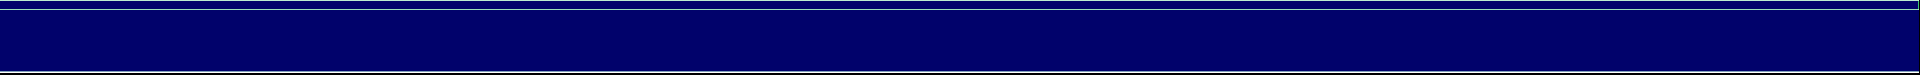
\includegraphics[height=0.9 true cm]{kekcsik.png}}

% ----------------------------------------------------------------------------------------------------------------------------------------

\begin{document}

\frame{\titlepage}

% ----------------------------------------------------------------------------------------------------------------------------------------

\begin{frame}[fragile,squeeze,allowframebreaks]
\frametitle{Where are we?}
\begin{itemize}
\setlength{\parskip}{0pt}
\setlength{\itemsep}{0pt}
\item \st{Motion of charged particles in electromagnetic fields.}
  \item \st{Elements of quantum mechanics. Heisenberg's uncertainty principle. The stationary Schrödinger equation and its applications.}
\item \st{Limits of the classical conceptual framework. Thermal radiation. Photoelectric effect. Compton effect. The dual nature of electromagnetic radiation. The dual nature of particles.}
\item \st{Moving reference frames. Inertial forces in accelerating reference frames. Elements of special relativity. Dirac-equation, antimatter.}
\item \st{The classical theory of atomic structure (Rutherford, Franck-Hertz experiment, Bohr model, quantum numbers, Pauli exclusion principle).}
\item \textbf{Physics of condensed matter. Metallic bonding. Electrical conduction in metals based on the free electron model and the wave model. Hall effect. Band theory of solids.}
\pagebreak
\item Semiconductors. Elements of Fermi-Dirac statistics. Thermoelectric phenomena. Magnetic properties.  
\item Ferroelectricity. Piezoelectricity and electrostriction. Liquid crystals. Superconductivity.
\item Luminescence. Lasers. Basic knowledge of nuclear physics. Basic knowledge of particle physics.
\end{itemize}
\end{frame}

% ----------------------------------------------------------------------------------------------------------------------------------------

%\title[Kondenzált Anyagok Fizikája]{Kondenzált anyagok fizikája}
%\section{Kristályfizika}

\begin{frame}%[fragile,squeeze,allowframebreaks]
  \frametitle{Physics of condensed matter - Crystal Physics}
\begin{columns}
  \begin{column}{0.6\textwidth} 
\begin{itemize}
\item Classification of condensed matter: glasses, crystalline materials, amorphous materials.
\item Crystalline materials (a): systems with symmetry; a symmetry unit repeats through the material.
\item Glasses (b): high-viscosity, supercooled liquids that solidify very slowly; produced by rapid cooling of a liquid state.
\item Amorphous materials: may contain small crystalline fragments or no regular crystalline structure at all.
\end{itemize}
\end{column}
\begin{column}{0.42\textwidth} 
  \begin{center}
   \includegraphics[width=0.9\linewidth]{images-20251027/20251027a-crystals_page3_img1.png}
\end{center}
\end{column}
\end{columns}
\end{frame}

% ----------------------------------------------------------------------------------------------------------------------------------------

\begin{frame}
\frametitle{Classification of Crystals}
\begin{columns}
\begin{column}{0.625\textwidth} 
\begin{itemize}
\item Ideal crystal: infinite extent with perfect symmetry.
\item Real crystal: ordered only in finite regions; contains lattice defects.
\item Single crystal (a): grown from one nucleation center under special conditions.
\item Polycrystal (b): grown from many nucleation centers; effectively a collection of many crystallits.
\item Macromolecular solids: built from giant molecules composed of many identical repeating units.
\end{itemize}
\end{column}
\begin{column}{0.42\textwidth} 
\begin{center}
\includegraphics[width=0.9\linewidth]{images-20251027/20251027a-crystals_page4_img1.png}
\end{center}
\end{column}
\end{columns}
\end{frame}

% ----------------------------------------------------------------------------------------------------------------------------------------

\begin{frame}
 \frametitle{Ideal Crystals and Unit Cells}
\begin{itemize}
\item Crystal lattices can be constructed from unit cells or lattice elements.
\item Translations fill space without gaps; lattice constant defines the translation length.
\end{itemize}
\begin{center}
\includegraphics[width=0.55\linewidth]{images-20251027/20251027a-crystals_page5_img1.jpeg}
\includegraphics[width=0.55\linewidth]{images-20251027/20251027a-crystals_page5_img2.jpeg}
\end{center}
\end{frame}

% ----------------------------------------------------------------------------------------------------------------------------------------

\begin{frame}[fragile,squeeze,allowframebreaks]
\frametitle{Bravais Lattices and Crystal Systems}
\begin{itemize}
\setlength{\parskip}{0pt}
\setlength{\itemsep}{0pt}
\item There are 7 crystal systems and 14 types of Bravais lattices.
\item Types of lattice centering:
\vskip -5 pt
\begin{itemize}
\setlength{\parskip}{0pt}
\setlength{\itemsep}{0pt}
\item \textbf{Primitive}: particles (atoms) are located only at the lattice points (corners of the cell).
\item \textbf{Body-centered}: an additional particle is located at the center of the cell.
\item \textbf{Base-centered}: particles are located at the centers of the top and bottom faces.
\item \textbf{Face-centered}: particles are located at the centers of all faces of the cell.
\end{itemize}
\vskip -5 pt
\item The seven crystal systems:
\begin{itemize}
\setlength{\parskip}{0pt}
\setlength{\itemsep}{0pt}
\item \textbf{Cubic} $\rightarrow a=b=c, \ \alpha=\beta=\gamma=90^{\circ}$ \hfill (primitive, body-, face-centered)
\item \textbf{Tetragonal} $\rightarrow a=b\ne c, \ \alpha=\beta=\gamma=90^{\circ}$ \hfill (primitive, body-centered)
\item \textbf{Orthorhombic} $\rightarrow a\ne b\ne c, \ \alpha=\beta=\gamma=90^{\circ}$ \hfill (primitive, body-, base-, face-centered)
\item \textbf{Triclinic} $\rightarrow a\ne b\ne c, \ \alpha\ne\beta\ne\gamma\ne90^{\circ}$ \hfill (primitive)
\item \textbf{Monoclinic} $\rightarrow a\ne b\ne c, \ \alpha=\gamma=90^{\circ}, \ \beta\ne90^{\circ}$ \hfill (primitive, base-centered)
 \pagebreak
\item \textbf{Trigonal (Rhombohedral)} $\rightarrow a=b=c, \ \alpha=\beta=\gamma\ne90^{\circ}$ \hfill (primitive)
\item \textbf{Hexagonal} $\rightarrow a=b\ne c, \ \alpha=\beta=90^{\circ}, \ \gamma=120^{\circ}$ \hfill (primitive)
\end{itemize}
\end{itemize}

%\pagebreak
\begin{center}
  % \includegraphics[width=0.99\linewidth]{images-20251027/20251027a-crystals_page7_img1_modified.png}
  \includegraphics[width=0.425\linewidth]{images-20251027/bravais.png}
\end{center}

\pagebreak
\begin{center}
\includegraphics[width=0.425\linewidth]{images-20251027/20251027a-crystals_page8_img1.jpeg}
\includegraphics[width=0.425\linewidth]{images-20251027/20251027a-crystals_page8_img2.jpeg}\\
Primitive and body-centered lattices.
\end{center}

\pagebreak
\begin{center}
\includegraphics[width=0.42\linewidth]{images-20251027/20251027a-crystals_page8_img3.jpeg}
\includegraphics[width=0.42\linewidth]{images-20251027/20251027a-crystals_page8_img4.jpeg}\\
Base-centered and face-centered lattices.
\end{center}
\end{frame}


% ----------------------------------------------------------------------------------------------------------------------------------------

\begin{frame}[fragile,squeeze,allowframebreaks]
\frametitle{Lattice Defects}
\begin{center}
\includegraphics[width=0.65\linewidth]{images-20251027/20251027a-crystals_page9_img1.jpeg}\\Point defects: interstitial atoms (blue), vacancies (missing atoms), substitutional impurities (red, green).
\end{center}

\pagebreak
\begin{center}
\includegraphics[width=0.65\linewidth]{images-20251027/20251027a-crystals_page10_img1.png}\\Frenkel defect: a vacancy and a self-interstitial created simultaneously.
\end{center}
\end{frame}

% ----------------------------------------------------------------------------------------------------------------------------------------

%\section{Band Theory (Sávelmélet)}

\begin{frame}
\frametitle{Band Theory -- Basics}
\begin{itemize}
  \item Use statistical descriptions for systems with many particles; electrons are fermions described by Fermi–Dirac statistics.
  \item Fermions have half-integer spin; Pauli exclusion principle applies: at most two electrons (with opposite spins) per quantum state.
  \item Phase-space cell concept: $\Delta p \cdot \Delta x$ finite quantum volume.
\end{itemize}
\end{frame}

% ----------------------------------------------------------------------------------------------------------------------------------------

\begin{frame}
\frametitle{Free Electron Model and Sommerfeld--Bloch}
\begin{itemize}
  \item Sommerfeld (1928) and Bloch (1930) developed the band model based on the free electron approximation.
  \item In a crystal, atomic levels split because nearby atoms interact; many atoms produce bands from originally discrete levels.
  \item In solids with very many atoms, split levels broaden into energy bands; allowed bands separated by forbidden gaps (band gaps).
\end{itemize}
\end{frame}

% ----------------------------------------------------------------------------------------------------------------------------------------

\begin{frame}[fragile,squeeze,allowframebreaks]
\frametitle{Example: Sodium (Na)}
\begin{center}
\includegraphics[width=0.8\linewidth]{images-20251027/PeriodicTableECBlocks.png}
\end{center}

\pagebreak
\begin{itemize}
 \item Single Na atom: electronic configuration 1s$^2$ 2s$^2$2p$^6$3s$^1$ (total of 11 electrons).
   \begin{columns}
     \begin{column}{0.25\textwidth}
       \begin{center}
         \includegraphics[width=0.9\linewidth]{images-20251027/20251027b-bands_page5_img1.jpeg}
         \end{center}
     \end{column}
     \begin{column}{0.65\textwidth}\vskip -10 pt
\begin{itemize}
\item Its electronic configuration (according to Bohr's postulates and the Pauli exclusion principle): 2 electrons on the first (K) shell, 8 on the second (L) shell, and 1 on the third (M) shell.
\item Representation of the electron configuration: according to the Pauli exclusion principle, a given level can hold a maximum of two electrons (with $s = +1$ or $s = -1$ spin quantum numbers on the same shell).
\item \textbf{M shell}, with its remaining 1 electron.\\
\textbf{L shell}, with 4 possible subshells, each containing 2 electrons — a total of 8 electrons maximum.\\
An atomic level. \textbf{K shell}, with 2 electrons.
\end{itemize}
\end{column}
\end{columns}

\pagebreak
\item Case of multiple Na atoms forming a Na crystal:
 \begin{columns}
     \begin{column}{0.25\textwidth}
       \begin{center}
         \includegraphics[width=0.9\linewidth]{images-20251027/20251027b-bands_page6_img1.jpeg}
         \end{center}
     \end{column}
     \begin{column}{0.8\textwidth}\vskip -15 pt
\begin{itemize}
\item When a crystal (a solid body) is formed from many individual Na atoms, the atoms influence each other — that is, they interact.
\item This interaction also affects the atomic energy levels, which themselves begin to influence one another.
\item As a result of these interactions, the atomic energy levels split (it can be shown that a level splits into as many sublevels as there are interacting atoms).
\item Therefore, the energy levels of a solid are determined by the collective energy levels of its constituent atoms:\\
   e.g., for 2 Na atoms:\\
   the \textbf{M shell} splits into 2 levels,\\
   the \textbf{L shell} splits into 8 levels,\\
   and the \textbf{K shell} splits into 2 levels.
\end{itemize}
\end{column}
\end{columns}

\pagebreak
\item For a system consisting of a large number of Na atoms:
\begin{columns}
     \begin{column}{0.375\textwidth}
       \begin{center}
         \includegraphics[width=0.9\linewidth]{images-20251027/20251027b-bands_page7_img1.png}
         \end{center}
     \end{column}
     \begin{column}{0.75\textwidth}\vskip -15 pt
\begin{itemize}
\item For a collection of at least $10^{9}$ atoms, the split energy levels broaden into bands. In this case, we speak of \textbf{energy bands}, or simply \textbf{bands}.
\item Because there are so many atoms in a crystal, the levels within a band effectively merge together.
\item In the band model, electrons can only occupy energies that fall within the allowed bands.
\item The allowed bands are separated by \textbf{forbidden bands} or \textbf{band gaps}. Electrons cannot exist in the energy states corresponding to forbidden bands.
\item Moving toward higher energies, the bands become wider because the influence of neighboring atomic nuclei also affects these electrons — this interaction stretches and broadens the bands.
\end{itemize}
\end{column}
\end{columns}

\pagebreak
\item For a system consisting of a large number of Na atoms:
\begin{columns}
     \begin{column}{0.4\textwidth}
       \begin{center}
         \includegraphics[width=0.9\linewidth]{images-20251027/20251027b-bands_page7_img1.png}
         \end{center}
     \end{column}
     \begin{column}{0.7\textwidth}\vskip -15 pt
\begin{itemize}
\item Electrons close to the nucleus are more strongly attracted and bound than the outer electrons. $\Rightarrow$ The inner electrons practically do not contribute to changes in the atom’s total energy. $\Rightarrow$ The lower bands correspond to smaller energies and are completely filled with electrons.
\item Interpretation (conduction band): The band above the highest completely filled energy band, which is either partially filled or empty, is called the \textbf{conduction band} (C). The conduction band is separated from the ground band by a \textbf{forbidden zone} (F).
\item The highest completely filled energy band is called the \textbf{ground band} (G). These are also referred to as the \textbf{valence bands}.
%\item  In a Na crystal, atomic levels split; for large numbers of atoms, broad energy bands form (valence band, conduction band).
%\item Valence band: highest completely filled band. Conduction band: band above the valence band, partially filled or empty.
%\item A forbidden gap separates the valence and conduction bands.
\end{itemize}
\end{column}
\end{columns}
\end{itemize}
\end{frame}

% ----------------------------------------------------------------------------------------------------------------------------------------

\begin{frame}[fragile,squeeze,allowframebreaks]
  \frametitle{Conductors, Insulators, Semiconductors}
The electrical properties of solids are determined by the relative positions of their uppermost energy bands. Depending on the position of these bands, solids can behave as conductors, insulators, or semiconductors.
  \begin{itemize}

\item Conductors: metals with an odd number of valence electrons have partially filled conduction bands.
 \begin{columns}
     \begin{column}{0.3\textwidth}
       \begin{center}
         \includegraphics[width=0.9\linewidth]{images-20251027/20251027b-bands_page10_img1.png}
         \end{center}
     \end{column}
     \begin{column}{0.8\textwidth}\vskip -15 pt
\begin{itemize}
\item In metals, each atom splits into a positive ion and an odd number of valence electrons.
\item Since the valence electrons are arranged in pairs within each energy level, the conduction band is only partially filled with electrons.
\item Allowed but unoccupied band.\\
Electron-filled band or portion of a band within the conduction band.\\
Electrons in the conduction band can absorb energy from an electric field and thus move from lower to higher energy levels. The disturbance of equilibrium in this way manifests as an electric current.
  \end{itemize}
\end{column}
\end{columns}

\pagebreak
\item Conductors: metals with an even number of valence electrons may have overlapping valence and conduction bands.
 \begin{columns}
     \begin{column}{0.4\textwidth}
       \begin{center}
         \includegraphics[width=0.9\linewidth]{images-20251027/20251027b-bands_page11_img1.jpeg}
         \end{center}
     \end{column}
     \begin{column}{0.6\textwidth}\vskip -15 pt
\begin{itemize}
\item Each atom splits into a positive ion and an even number of electrons.
\item The electrons occupy energy levels in pairs and completely fill the valence band.
\item The conduction band of these metals is completely empty but overlaps partially with the valence band — that is, there is no forbidden band between the valence (V) and conduction (C) bands.
\item Electrons can easily absorb energy from an electric field, enabling electrical conduction.
  \end{itemize}
\end{column}
\end{columns}

\pagebreak
  \item Insulators: large band gap (2–10 eV) prevents thermal excitation of electrons into the conduction band. If the forbidden band between the fully filled valence band and the completely empty conduction band is wide — i.e., between 2 and 10 eV — the solid behaves as an insulator.
\begin{columns}
     \begin{column}{0.4\textwidth}
       \begin{center}
         \includegraphics[width=0.9\linewidth]{images-20251027/20251027b-bands_page12_img1.jpeg}
         \end{center}
     \end{column}
     \begin{column}{0.75\textwidth}\vskip -15 pt
\begin{itemize}
\item Does not conduct electric current.
\item Electrons in the valence band cannot gain enough energy from an electric field to jump across the forbidden band into the conduction band.
\item Electrons cannot acquire this energy thermally either. The crystal would melt before becoming conductive in the solid state.
\end{itemize}
\end{column}
\end{columns}

\pagebreak
\item Semiconductors: narrow band gap (a few tenths of an eV); thermal excitation of charge carriers strongly depends on temperature. If the forbidden band between the completely filled valence band and the empty conduction band is only a few tenths of an eV wide, the crystal behaves as an insulator at low temperatures, but its electrical conductivity increases with rising temperature.
\begin{columns}
     \begin{column}{0.4\textwidth}
       \begin{center}
         \includegraphics[width=0.9\linewidth]{images-20251027/20251027b-bands_page13_img1.png}
         \end{center}
     \end{column}
     \begin{column}{0.7\textwidth}\vskip -15 pt
\begin{itemize}
\item Due to thermal excitation, electrons in the valence band can jump across the very narrow forbidden band into the conduction band.
\item Since the number of electrons crossing into the conduction band is small and highly temperature-dependent, the resulting current is weak and also temperature-dependent. Semiconductors with such properties are called \textbf{intrinsic semiconductors}.
\end{itemize}
\end{column}
\end{columns}

\end{itemize}
\end{frame}

% ----------------------------------------------------------------------------------------------------------------------------------------

\begin{frame}[fragile,squeeze,allowframebreaks]
\frametitle{Wave Model and Forbidden Wavelengths}
\begin{itemize}
\item Electrons can be treated as waves in the crystal; standing waves (arising from reflections on lattice planes) are forbidden for conduction electrons.\\
\begin{center}
\includegraphics[width=0.75\linewidth]{images-20251027/20251027b-bands_page15_img1.jpeg}
\end{center}
\item Due to interference, maximum reinforcement occurs when: $d \cdot \sin\alpha = n \cdot \frac{\lambda}{2}$.
\item Multiplying both sides by 2: $2d \cdot \sin\alpha = n \cdot \lambda$.
\item If $\alpha = 90^{\circ}$, the condition for interference becomes: $2d = n \cdot \lambda \rightarrow \lambda = \frac{2d}{n}, \ n = 1, 2, 3, \dots$.
\item The physical meaning of this interference condition: formation of standing waves.
\item The formation of standing waves is forbidden for conduction electrons because a standing wave is not a traveling wave — and conduction electrons are identified with traveling waves.
\item Therefore, the forbidden wavelengths are: $\lambda_{forbidden} = \frac{2d}{n}, \ n = 1, 2, 3, \dots$
\item Let us write the de Broglie equation for these forbidden wavelengths: 
$$\mathbf{Forbidden\ momenta:} \quad p_{forbidden} = \frac{h}{\lambda} = \frac{nh}{2d}.$$
\pagebreak
\item The kinetic energy of free electrons is:
$$W_{kin} = \frac{1}{2}mv^{2} = \frac{p^{2}}{2m},$$ 
since $p = mv$.
\item If we express the kinetic energy using the forbidden momenta:
$$\mathbf{Forbidden\ energy:} \quad W_{kin-forbidden} = \frac{p_{t}^{2}}{2m} = \frac{n^{2}h^{2}}{4d^{2} \cdot 2m} = \frac{n^{2}h^{2}}{8md^{2}}.$$
\item These forbidden energies give rise to forbidden or band-gap energy regions.
  \pagebreak
\item From $W_{kin} = \frac{p^{2}}{2m}$ we obtain a parabolic relation (dashed line: allowed region, empty: forbidden region).
\begin{center}
  \includegraphics[width=0.465\linewidth]{images-20251027/20251027b-bands_page17_img1.jpeg}
\end{center}
\item The conduction electrons (valence electrons) cannot have such so-called forbidden energies that fall within the forbidden energy bands. That is, electrons cannot exist in forbidden bands.

  \pagebreak
\item The properties of crystals are determined by the occupancy of allowed energy bands, the width of the forbidden bands, and their relative positions.\\
$\Rightarrow$ Conductors, insulators, and semiconductors can be defined — in terms of electrical conductivity — by the relative arrangement of forbidden bands and allowed valence and conduction bands, as seen in the free-electron model.\\
$\Rightarrow$ Both models lead to the same conclusion.
\begin{center}
  \includegraphics[width=0.65\linewidth]{images-20251027/20251027b-bands_page18_img1.png}
\end{center}
\end{itemize}
\end{frame}

% ----------------------------------------------------------------------------------------------------------------------------------------

%\section{Metallic Bonding and Hall Effect}

\begin{frame}[fragile,squeeze,allowframebreaks]
\frametitle{Metallic Bonding -- Free Electron Model}
\begin{itemize}
\item Metallic bond: metal ions occupy lattice sites, and delocalized electrons move freely through the lattice (electron gas model).
\begin{center}
\includegraphics[width=0.7\linewidth]{images-20251027/20251027c-metal_hall_page3_img1.png}
\end{center}

\pagebreak
\item Energy (W) and forces (F) in the crystal lattice.
\item Types of lattices: ionic lattice, atomic lattice, molecular lattice.
\item The particles occupy those positions in the lattice where the resultant force is zero.
\item Where the resultant force is zero, the energy has a local minimum.
\begin{center}
\includegraphics[width=0.7\linewidth]{images-20251027/20251027c-metal_hall_page4_img1.png}
\end{center}

\pagebreak
\item Metallic bonding: metal ions are located at the lattice sites, and free (delocalized) electrons move between them.
\item Details of metallic bonding illustrated through the example of sodium.
\item Case of sodium vapor: bound electronic state. It consists of sodium atoms located far from each other.
\begin{center}
\includegraphics[width=0.675\linewidth]{images-20251027/20251027c-metal_hall_page5_img1.png}
\end{center}

\pagebreak
\item Case of metallic sodium: the 3s (1) electron is no longer bound to the atom. It can move freely within the crystal. $\Rightarrow$ Free electron model.
\item The free electrons perform thermal motion, similar to gas particles. $\Rightarrow$ Electron gas.
\begin{center}
\includegraphics[width=0.675\linewidth]{images-20251027/20251027c-metal_hall_page6_img1.png}
\end{center}

\end{itemize}
\end{frame}

% ----------------------------------------------------------------------------------------------------------------------------------------

\begin{frame}[fragile,squeeze,allowframebreaks]
 \frametitle{Conductivity in the Free Electron Picture}
\begin{itemize}
\item According to the equipartition theorem: $$\frac{1}{2}mv_{th}^{2}=\frac{3}{2}kT.$$
\item Average thermal velocity: $v_{\mathrm{th}} = \sqrt{3kT/m}$.
\item The average thermal velocity is proportional to the square root of the absolute temperature.
\item When an electric field is applied to the metal, the motion of the electrons becomes directed: $$\mathbf{F}=m\mathbf{a}, \quad \mathbf{F}=-e\mathbf{E}.$$
 \pagebreak
\item Therefore: $$\mathbf{a}=\frac{\mathbf{F}}{m}=\frac{-e\mathbf{E}}{m},$$ where $e$ is the electron charge, $m$ is the electron mass, $\mathbf{E}$ is the electric field vector, $\mathbf{F}$ is the force, and $\mathbf{a}$ is the acceleration.
\item The electrons undergo collisions. Let $t$ be the time interval between two collisions, and let $l_{k}$ be the mean free path between collisions. Then the velocity magnitude is:  
$$v=a\cdot t=\frac{eE}{m}\frac{l_{k}}{v_{th}}.$$
\item The average velocity, or drift velocity, is defined as: $$v_{avg}=\frac{v}{2}.$$
\pagebreak
\item Substituting the expression for $v$, we obtain: $$v_{avg}=\frac{eE}{2m}\frac{l_{k}}{v_{th}}.$$
\item Let us now express the electric current density ($J$) in the metal.
\item By definition, the electric current density is the number of charges (charge carriers — electrons) crossing a unit area per unit time.
\item Thus: $$J=\frac{Q}{A\cdot t}=\frac{n\cdot e\cdot v_{avg}\cdot t\cdot A}{A\cdot t}=n\cdot e\cdot v_{avg}.$$
\pagebreak
\item Define the electrical resistivity ($\rho$) as the magnitude of the electric field that produces a unit current density:  
$$\rho=\frac{E}{J}=\frac{E}{n\cdot e\cdot v_{avg}}.$$
\item Since the electrical conductivity ($\gamma$) is the reciprocal of resistivity, we have:  
$$\gamma=\frac{1}{\rho}=\frac{J}{E}=\frac{n\cdot e\cdot v_{avg}}{E}=\frac{n\cdot e\cdot \frac{eE}{2m}\cdot\frac{l_{k}}{v_{th}}}{E},$$  
that is,  
$$\gamma=\frac{n\cdot e^{2}\cdot l_{k}}{2m v_{th}} \Rightarrow \gamma \sim \frac{1}{v_{th}}.$$
\item However, since $v_{th} =\sqrt{\frac{3kT}{m}}$, we have $v_{th}\sim\sqrt{T}$. Therefore:  
$$\gamma\sim\frac{1}{\sqrt{T}}.$$
\item In this model, the electrical conductivity is inversely proportional to the square root of the absolute temperature. However, it is now known that the resistivity of metals is approximately a linear function of temperature, and the conductivity is inversely proportional to it.
\end{itemize}
\end{frame}

% ----------------------------------------------------------------------------------------------------------------------------------------

\begin{frame}
\frametitle{Conductivity -- Wave Model Perspective}
\begin{itemize}
\item According to the wave model, the freely moving electrons in a metallic crystal lattice can be represented as waves.
\item In metals, the electron waves are scattered by density fluctuations caused by lattice vibrations, as well as by possible impurities, leading to scattering on these density fluctuations or impurity sites.
\item From Sommerfeld’s theory, it can be shown that  
$$\gamma \sim \frac{1}{T}.$$
\end{itemize}
\end{frame}


% ----------------------------------------------------------------------------------------------------------------------------------------

\begin{frame}[fragile,squeeze,allowframebreaks]
\frametitle{Hall Effect — Description}
\begin{itemize}
\begin{columns}
\begin{column}{0.4\textwidth}
\item When a current-carrying metal plate is placed in a magnetic field, a transverse electric field (Hall field) appears, which is perpendicular to both the current density and the magnetic induction.
\end{column}
\begin{column}{0.45\textwidth}
\begin{center}
\includegraphics[width=0.9\linewidth]{images-20251027/20251027c-metal_hall_page15_img1.jpeg}
\end{center}
\end{column}
\end{columns}

\pagebreak
\item Lorentz force: the magnetic component of the electromagnetic force causes charge separation.
\item Hall voltage: $U_H = R_H \frac{I B}{d}$, where $R_H = \frac{1}{n e}$ is the Hall coefficient (in the simple single-carrier model).

\item The Lorentz force acting on an elementary charge moving in an electromagnetic field is:  
$$\mathbf{F} = e\mathbf{E} + e\left(\mathbf{v} \times \mathbf{B}\right).$$
\item For a charge moving only in a magnetic field:  
  $$F = e\left(\mathbf{v} \times \mathbf{B}\right).$$

 \pagebreak
\item Due to the Lorentz force, the charges in the plate are deflected in a direction perpendicular to both the magnetic induction and their velocity. As a result, charges accumulate on the two opposite sides of the sample, leading to charge separation.
\item As a consequence of this charge separation, an electric field builds up between the separated charges. Thus, for these charges:  
$$\mathbf{F} = e\mathbf{E}.$$
\item Therefore,  
  $$evB = eE, \quad vB = E.$$

\pagebreak  
\item The current density vector is given by:  
$$\mathbf{J} = n e \mathbf{v}.$$
\item Considering that for a plate of thickness $d$ and width $b$, the current and current density are related by:  
$$J = \frac{I}{A} = \frac{I}{b d}.$$
\item We also know that:  
$$U_H = E b.$$
\item Combining the above relations:  
$$E = \frac{U_H}{b} = vB = \frac{J}{n e}B = \frac{I}{n e b d}B.$$

\pagebreak
\item From this expression, the Hall voltage can be written as:  
$$U_H = \frac{1}{n e} \frac{I B}{d} = R_H \frac{I B}{d}.$$
\item The resulting voltage is called the \textbf{Hall voltage}.
\item The constant $R_H$ is a material-specific parameter called the \textbf{Hall coefficient}.
\end{itemize}
\end{frame}

% ----------------------------------------------------------------------------------------------------------------------------------------

\begin{frame}
%\frametitle{Minden jó, ha a vége jó}

\vfill
\begin{center}
\textbf{\huge The End}

\bigskip
Thank you for your attention!
\end{center}
\vfill
\end{frame}

\end{document}
